% This is part of Mes notes de mathématique
% Copyright (c) 2011-2012
%   Laurent Claessens
% See the file fdl-1.3.txt for copying conditions.

\thispagestyle{empty}
\begin{center}
  \begin{minipage}{15cm}
    \hrule\par
    \vspace{2mm}
    \begin{center}
    \Huge \bfseries Mes notes de mathématique \par
    \end{center}
    \hrule\par
  \end{minipage}
\end{center}

\vspace{2cm}

\begin{center}
    Laurent \textsc{Claessens}\\
    %Université libre de Bruxelles (2008-2009)\\
    %Université catholique de Louvain (2009-2010)\\
    %Université de Franche-Comté (2010-2012)\\
    \ifthenelse{\value{isAgreg}=0}{\today}{2012}\\
    \url{http://student.ulb.ac.be/~lclaesse/mes_notes2012-provisoire.pdf}\\
    \url{http://student.ulb.ac.be/~lclaesse/mes_notes.pdf}
\end{center}

\vfill

\ifthenelse{\value{isAgreg}=0}{
\begin{center}

           \ifpdf
            
\includegraphics[width=1cm]{gfdl-logo-small.png}
        \else
            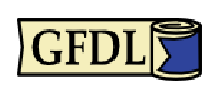
\includegraphics[width=1cm]{gfdl-logo-small.eps}
        \fi

Copyright (c) 2011-2012  Laurent Claessens, Carlotta Donadello, Djèlil Chafaï

Permission is granted to copy, distribute and/or modify this document under the terms of the \href{http://www.gnu.org/licenses/fdl-1.3.html}{GNU Free Documentation License}, Version 1.3 or any later version published by the Free Software Foundation; with no Invariant Sections, no Front-Cover Texts, and no Back-Cover Texts. A copy of the license is included in the chapter entitled ``GNU Free Documentation~License''.

\vspace{0.5cm}

Vous avez le droit de copier, distribuer et modifier ce document pourvu que vous suiviez les règles de la \href{http://www.gnu.org/licenses/fdl-1.3.html}{GNU Free Documentation License}. Vous trouverez les sources \LaTeX\ à l'adresse\\ \url{https://www.gitorious.org/mes-notes-de-math-matique}

\end{center}
} 
{
    \TextePourISBN

}

% Ajouter ici l'ISBN. Pour les révisions, mettre un nouvel ISBN et indiquer que c'est une révision.
% Pour l'ISBN:
% Copier tout dans un nouveau répertoire
% Créer une nouvelle branche git
% Coder en dur la date (càd enlever \today)
% Changer la licence vers non modifiable, copiable, et ajouter un lien vers la version modifiable.
% Enlever les couleurs, en particulier les URL et les liens internes.

% http://www.bnf.fr/fr/professionnels/s_informer_obtenir_isbn/s.qu_est_ce_que_isbn.html

% Il faut écrire l'ISBN au verso de la page de titre, au bas de la dernière page de couverture et au bas de la dernière page de la jaquette des livres ;


% TODO: écrire le README.txt

% De temps en temps, il faut renvoyer une nouvelle version à
% http://megamaths.perso.neuf.fr/

\clearpage

% Ceci est pour avoir l'ISBN au dos de la dernière page de couverture.


\clearpage

%+++++++++++++++++++++++++++++++++++++++++++++++++++++++++++++++++++++++++++++++++++++++++++++++++++++++++++++++++++++++++++
\section*{Auteurs, contributeurs et remerciements}
%+++++++++++++++++++++++++++++++++++++++++++++++++++++++++++++++++++++++++++++++++++++++++++++++++++++++++++++++++++++++++++

\begin{enumerate}
    \item Carlotta Donadello pour la partie géométrie analytique : topologie dans \( \eR^n\), courbes, intégrales, limites. (Université de Franche-Comté 2010-2012)
    \item Djalil Chafaï pour toute la partie qui porte son nom. Plus généralement pour tout ce que je me suis permis de pomper chez lui :\\ \href{http://djalil.chafai.net/enseignement.html}{http://djalil.chafai.net/enseignement.html} Une soixantaine de pages lui sont dues. Je me suis permis de retirer cependant toutes ses références à matlab et autres logiciels que je ne maîtrise pas, afin de ne laisser que Sage.
    \item Nicolas Richard et Ivik Swan pour les parties des exercices et rappels de calcul différentiel et intégral (Université libre de Bruxelles, 2003-2004) qui leur reviennent.
    \item Pierre Bieliavsky pour les énoncés d'analyse numérique (MAT1151 à Louvain la Neuve 2009-2010)
    \item Jonathan Di Cosmo pour certaines corrections de MAT1151
    \item
        Mihai Bostan nous a donné ses notes manuscrites de son cours présentiel de géométrie analytique 2009-2010. (presque) Toute la structure du cours de gémétrie analytique lui est due (qui est maintenant fondue un peu partout dans les chapitres d'analyse).
    \item
        François Lemeux, exercices sur les normes de matrices et correction de coquilles.
    \item
        Les étudiants de géométrie analytique en CTU 2010-2011 ont détectés d'innombrables coquilles.
    \item
        Les étudiants du cours présentiel de géométrie analytique 2011-2012 ont signalé un certain nombre d'incorrections dans les exercices et les corrigés.
    \item
        Mustapha Mokhtar-Kharroubi pour la matière et la structure du cours de outils mathématiques.
    \item
        Martin Meyer et Mustapha Mokhtar-Kharroubi pour certains exercices de outils mathématiques (surtout ceux des DS et examens).
    \item
        Tous les contributeurs du wikipédia francophone (et aussi un peu l'anglophone) doivent être remerciés. J'en ai pompé des quantités astronomiques; des articles utilisés sont cités à divers endroits du texte, mais ce n'est absolument pas exhaustif. Il n'y a à peu près pas un résultat important de ces notes dont je n'aie pas lu la page Wikipédia, et souvent plusieurs pages connexes.
    \item
        Des centaines de profs qui ont mis leurs polys sur internet. Des dizaines d'entre eux et entre elles ont des sites dédiés à l'agrégation. Ils sont cités en bibliographie aux endroits où ils sont utilisés. Merci à toutes et à tous d'avoir codé et publié. Encore plus merci à celles et ceux qui ont pris la peine de préciser une licence et merci spécial pour les licences libres (quant à ceux dont la licence libre couvre également le code \LaTeX\ publié \ldots).
    \item
        Le forum usenet de math, en particulier pour la construction des corps fini dans la fil «Vérifier qu'un polynôme est primitif» initié le 20 décembre 2011.
    \item
        Le forum usenet de \LaTeX\ pour de nombreuses choses.
    \item
        Les intervenants du fil «\href{http://www.les-mathematiques.net/phorum/read.php?2,302266}{Antisymétrisation, alterné, déterminant et caractéristique}» sur les-mathematiques.net m'ont bien aidé pour la section sur les déterminants \ref{SecGYzHWs} (bien qu'ils ne le savent pas).
\end{enumerate}

J'ai souvent donné entre parenthèse à côté des mots «théorème», «lemme» ou «proposition» une ou plusieurs références vers les sources de la preuve que je donne. Ce sont parfois des liens vers la bibliographie; parfois aussi des liens hypertexte vers des sites, des blogs, etc. Tous ces gens ont fait du bon boulot. Sans toute cette «communauté», l'internet serait mort\ifthenelse{\value{isAgreg}=0}{Cette dernière phrase doit être comprise comme un appel à ne pas utiliser Moodle et autres iCampus pour diffuser vos cours de math.}{}.

%Bien entendu les ouvrages de la bibliographie qui sont des livres publiés chez des éditeurs commerciaux sont exclus de ces remerciements. Dans les relations commerciales, le payement fait office de remerciements.
% Hein ? Il y a des auteurs qui ont réussi le double coup de 1. me faire payer pour lire leur prose et 2. ne pas toucher d'argent de ma part ? Est-il possible que le lien entre les auteurs et les lecteurs via un éditeur commercial soit à ce point perdant-perdant ? Ça se saurait ;)
